\part{Soluções Apresentadas}
\chapter[Introdução]{Introdução}
Neste capítulo abordaremos todas as soluções idealizadas para o projeto. O capítulo está dividido conforme os grupos descritos na subseção ~\ref{subsec:divisao}.

\chapter[Estruturas e Materiais]{Estruturas e Materiais}
\section{Otimização da Planta}
Neste projeto, foi utilizada como base a planta baixa dos prédios já existentes na Faculdade do Gama, Universidade de Brasília. Porém foi observado que seriam necessárias algumas mudanças para alcançarmos nossos objetivos com este projeto. Salas de aula serão alteradas de forma a otimizar tanto luminosidade, quanto ventilação; e laboratórios serão acrescentados no projeto visto que é perceptível a insuficiência do número de laboratórios numa faculdade de engenharias que possui alta demanda.

Similarmente, para realizar este projeto, foi necessária uma adaptação de elementos relativos a automação predial à um projeto de construção civil comum com integração do sistema Smart Grid, dando ênfase na sustentabilidade.
Um sistema de automação pode ser centralizado ou distribuído. Os centralizados são aqueles que utilizam uma seção especificamente para o controle dos dispositivos, tanto para receber quanto enviar sinais. Os sistemas distribuídos são considerados descentralizados porque utilizam de diversos dispositivos, cada um com uma função específica dentro do sistema, sendo distribuídos por toda instalação e interligados por uma rede \cite{dias22004}.

Considerando que a rede de automação a ser implementada possui um sistema centralizado, viu-se a necessidade de um local específico para controlar e monitorar o sistema. Já para promover a integração do Smart Grid ao projeto, foi constatado que o melhor ponto para a instalação das placas fotovoltaicas seria no telhado, onde há maior contato com sol, menor projeção de sombras e resguardado de contato de animais e pessoas. Quanto à posição da placa, esta deverá estar voltada para o norte.

Por mais que a representação da parte estrutural do projeto pudesse ser feita a mão, através de desenho técnico, viu-se a necessidade de realizar uma representação mais para que se possa realizar uma análise estrutural. Sendo assim, para garantir que os materiais escolhidos vão suprir as necessidades estruturais serão desenvolvidos, com a ajuda de softwares, o modelo 3D do prédio e a simulação dos esforços.
Foram levantadas algumas possibilidades para a utilização dos softwares, visto que há uma gama de opções. Para elaboração dos desenhos tanto em 2D, quanto em 3D, e sua renderização, estamos considerando a utilização do “AutoCad”, do “SketchUp” e o “Revit”. Para a simulação, o “ANSYS" será considerado.

Em relação ao “SketchUp” é levado em conta a facilidade na utilização do programa, e o fato de sua biblioteca online de modelagem de interiores ser bem completa. Quanto ao Revit, é um programa que tem melhor aplicação para modelagens arquitetônicas, hidráulicas e elétricas. O AutoCAD é semelhante ao Revit, porém é necessário que as etapas do desenho sejam feitas separadamente.

Para definir qual será utilizado, será levado em consideração o programa que suprir as necessidades do projeto da melhor forma. Serão analisados quesitos como facilidade de aquisição, facilidade de utilização, biblioteca, melhores ferramentas.

 \begin{figure}[!h]
 	\centering	\includegraphics[keepaspectratio=true,scale=0.3]{figuras/planta1.eps}
 	\caption{Planta Baixa - Primeiro Pavimento}
 	\label{fig02243}
\end{figure}

 \begin{figure}[!h]
 	\centering
\includegraphics[keepaspectratio=true,scale=0.3]{figuras/planta2.eps}
 	\caption{Planta Baixa - Térreo}
 	\label{fig02242}
\end{figure}

\pagebreak

Um dos requisitos deste prédio é que seja uma estrutura inteligente e que aproveite ao máximo os recursos disponíveis, tal como a luz natural proveniente do sol. Para tal, a disposição do prédio em relação à posição do sol é de extrema importância para que se possa ter o máximo proveito dentro do ambiente do prédio, garantindo a economia de energia elétrica. Visto que o Brasil localiza-se no hemisfério sul a melhor opção é posicioná-lo voltado para o norte geográfico, o qual garante maior taxa de iluminação natural ao longo do dia.

Alguns fatores devem ser levados em consideração, como o conforto visual, que é definido como condições pela qual um ser humano consiga exercer atividades em determinado ambiente sem forçar suas vistas \cite{garrocho2005}.

Para que o projeto possa ter uma boa iluminação natural, é necessário que se tenha aberturas ou materiais que permitem a passagem de luz, de modo que a luz penetre no recinto e se tenha a luminância bem distribuída na área desejada. Outro fator que deve ser levado em consideração para a otimização da iluminação na estrutura é o índice de luz solar que predomina na Faculdade do Gama ao longo do ano. Para isso, tem-se a representação gráfica abaixo:

 \begin{figure}[!h]
 	\centering
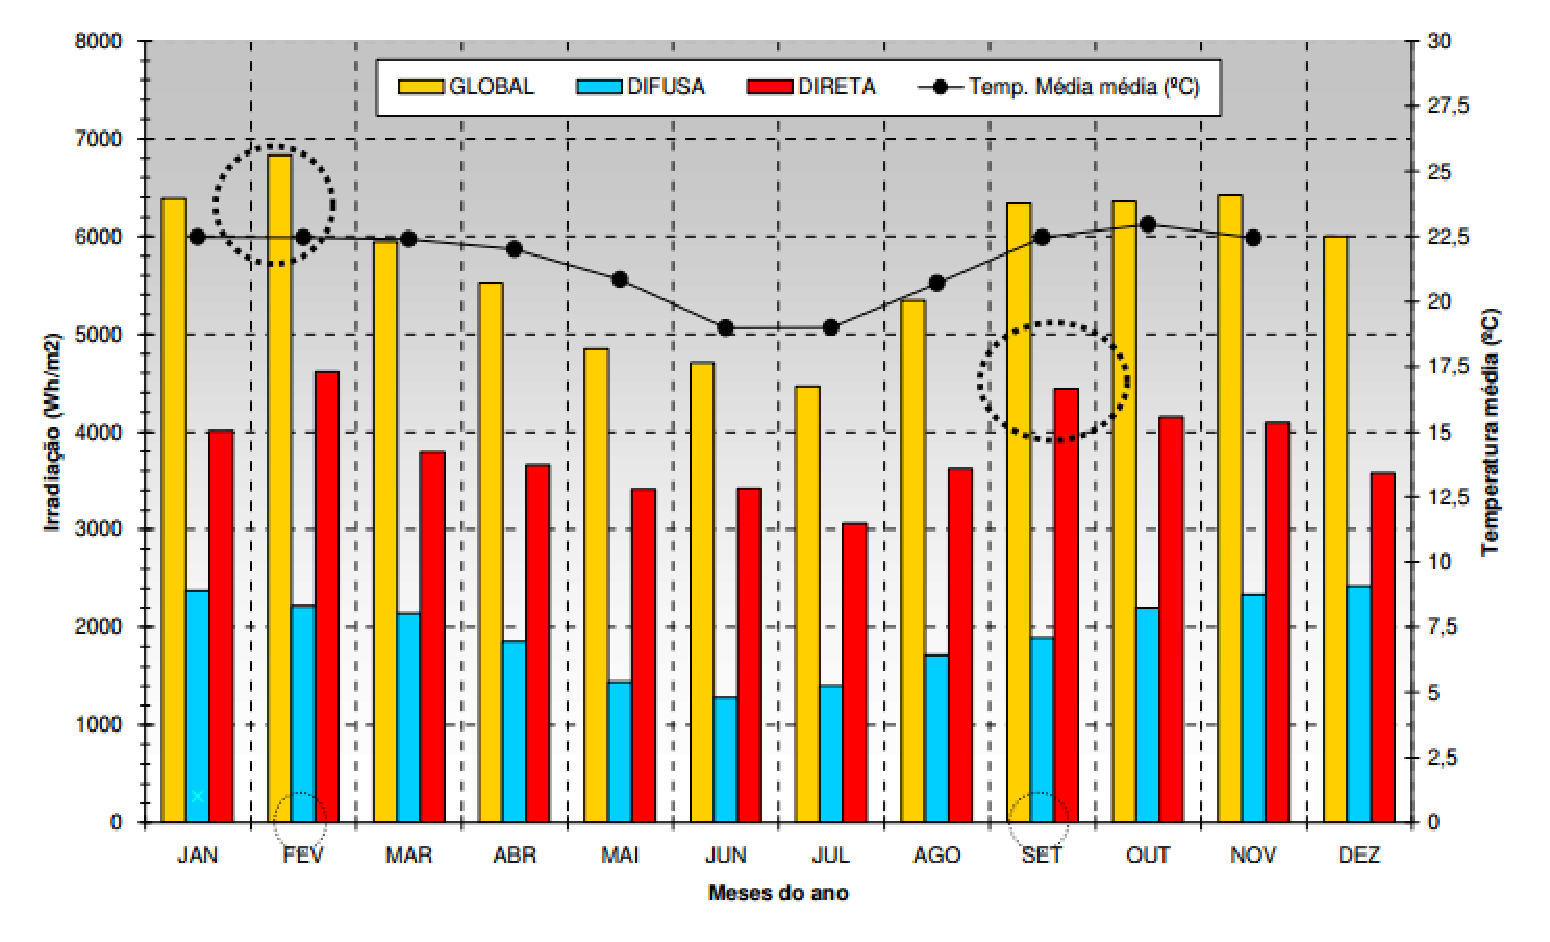
\includegraphics[keepaspectratio=true,scale=0.6]{figuras/luz.eps}
 	\caption{Nível de luz solar incidente em um plano horizontal em Brasília}
 	\label{fig02242}
\end{figure}

Além da iluminação, outro fator influencia diretamente no conforto dos estudantes do Campus:  a ventilação no ambiente da salas de aula. Nos prédios já construídos, um dos problemas mais relatados por parte dos alunos foi a má ventilação em sala de aula, visto que há pouco ar circulando, o que gera a sensação de calor e desconforto durante as aulas, principalmente em períodos no qual a temperatura de Brasília é mais elevada, ocasionando um ambiente abafado e incômodo para se estudar.

Para amenizar esse problema, é possível usar de uma propriedade física para conseguir uma ventilação natural, que é a utilização do efeito chaminé. Esse, consiste em ter abertura em diferentes níveis, de forma que faça com que o ar circule através de correntes de convecção, ou seja, o ar mais quente por ter uma densidade menor que o ar mais frio irá subir e se dispersar na abertura superior, de forma que elimina o calor presente no ambiente e ainda mantém a circulação de ar dentro do ambiente, de uma forma que além de natural, é barata.

 \begin{figure}[!h]
 	\centering
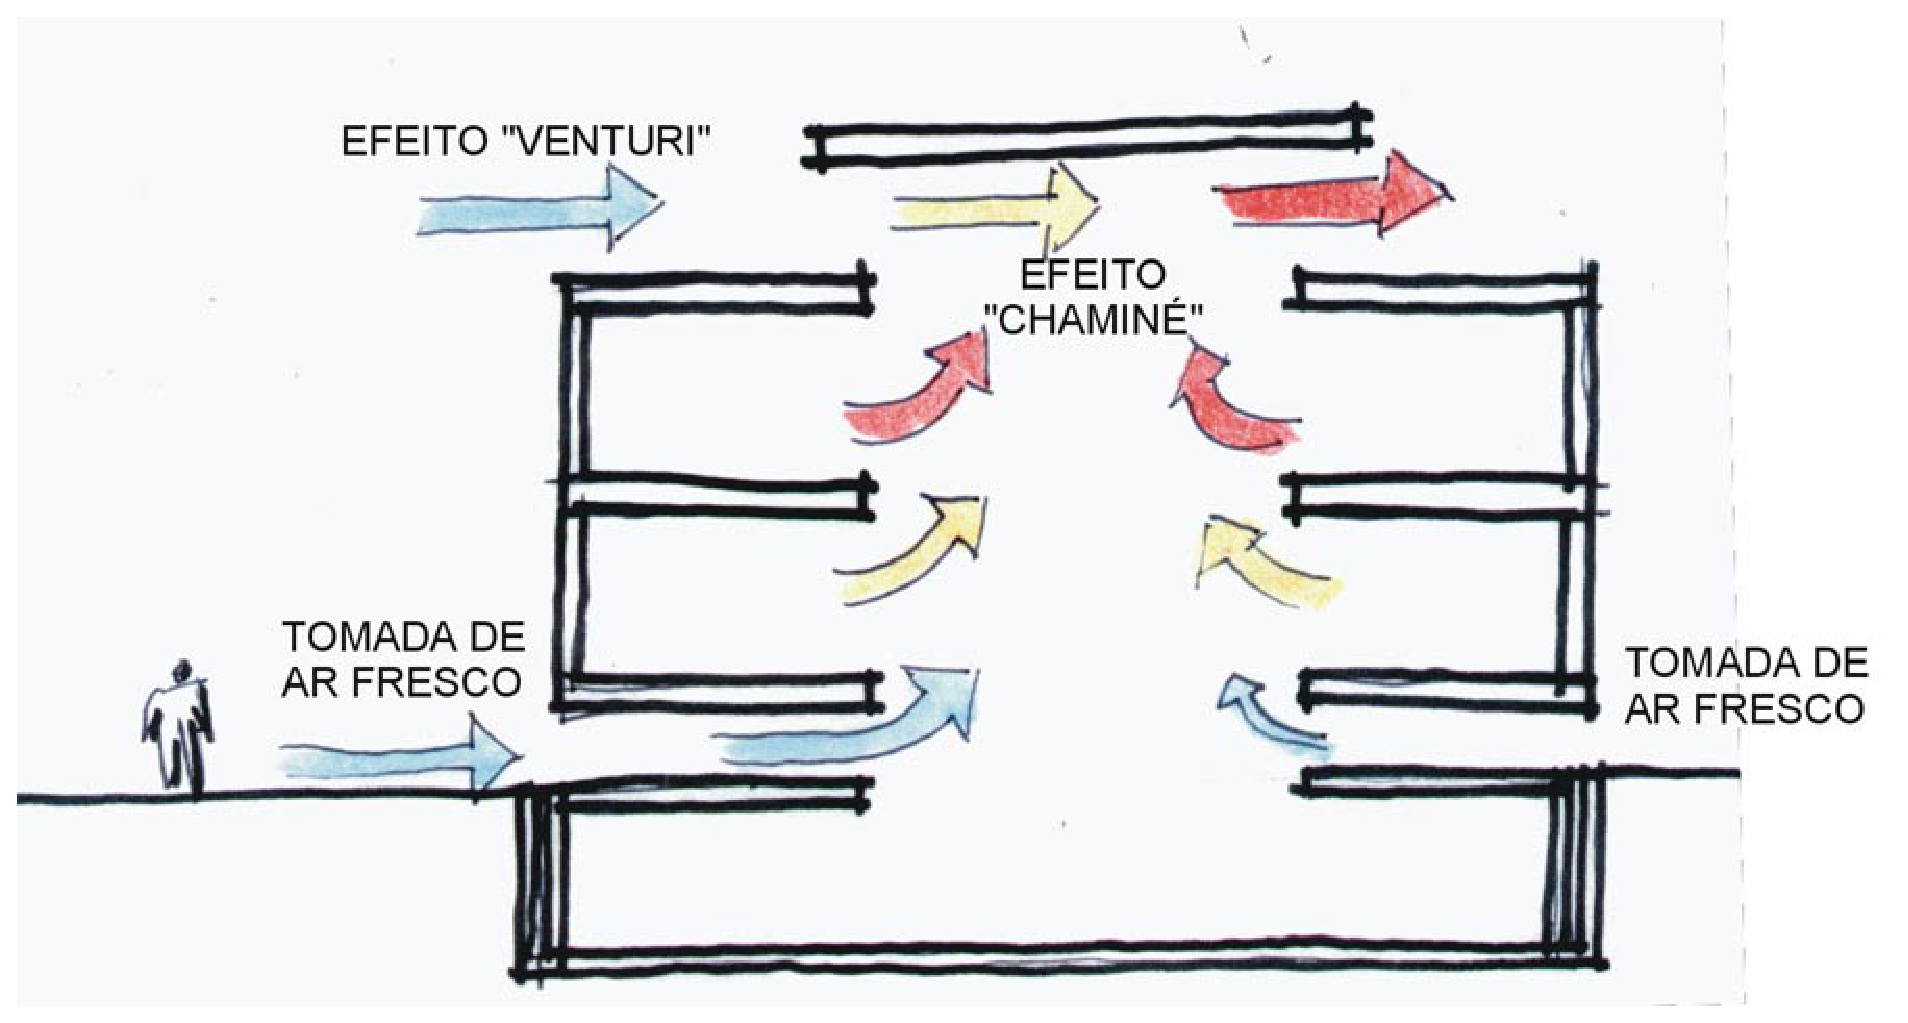
\includegraphics[keepaspectratio=true,scale=0.45]{figuras/chamine.eps}
 	\caption{Representação do efeito chaminé}
 	\label{fig02242}
\end{figure}

\section{Organização Interna}

Um dos problemas que o atual prédio de salas de aula da FGA enfrenta é o mau posicionamento dos quadros. Em muitas salas o quadro está muito alto forçando o professor a usar um tablado para alcançar o mesmo e em outras salas está tão baixo que é necessário que o professor só use da metade para cima. Segundo \cite{moro2005} o mobiliário da sala de aula como outros fatores físicos ,são grandes influenciadores no desempenho, segurança, conforto e comportamento dos alunos. Assim \cite{luz2005} afirma que um quadro mal posicionado pode ocasionar o esgotamento dos pequenos músculos ligados aos globos oculares,podendo causar tensão e desconforto em graus mais avançados.

 \begin{figure}[!h]
 	\centering
\includegraphics[keepaspectratio=true,scale=0.25]{figuras/projetor.eps}
 	\caption{Local onde são projetadas as imagens de powerpoint}
 	\label{fig02242}
\end{figure}

Desta forma podemos também fazer um comparativo com a posição dos projetores. Muitas vezes quando o professor utiliza o powerpoint, a imagem projetada apresenta baixa nitidez devido a luminosidade que entra pelas janelas e muitas vezes há complicações para enxergar uma parte da imagem que fica entre o quadro e a parede. Outro agravante é a necessidade de subir em carteiras para ligar e desligar esses equipamentos, o que pode comprometer a segurança dos usuários.

Para a questão da projeção da imagem, a solução consiste em colocar a lona de projeção e o projetor em um local da sala cuja luminosidade proveniente das janelas não atrapalhe a imagem projetada. Já para ligar o dispositivo, a solução deste problema é a extensão do mecanismo que liga e desliga o projetor para um local próximo ao professor, onde ficam os cabos que conectam o projetor ao computador.

O posicionamento das carteiras em sala de aula é dependente do posicionamento do quadro e projetor. Em grande parte das salas de aula as turmas são muito grandes, então os alunos que escolhem um assento no fundo da sala tem uma dificuldade para enxergar o quadro. A solução para esse problema é a construção de um tablado de madeira com vários níveis similar a um anfiteatro, mas adaptado para as dimensões da sala. Assim, todos os alunos vão ter acesso visual ao quadro.

Assim, a compreensão do conteúdo de sala de aula pode acabar sendo prejudicada pelos ruídos. Desta forma \cite{russo1999} diz que:
\begin{citacao}
Algumas vezes, essa tarefa pode ser comprometida pela intensidade insuficiente ou exagerada da voz do professor, por problemas de articulação, dificuldade de pronúncia ou vocabulário desconhecido, ou pela ausência da pista visual, quando o professor está escrevendo na lousa, voltando as costas para os alunos. Outras vezes é o ruído excessivo, tanto no interior quanto fora da sala de aula, nos corredores da escola, que exerce um efeito mascarante deletério sobre a mensagem falada.
\end{citacao}

Tendo em mente esse conceitos uma forma inicial para a amenização do problema acústico da sala de aula é a instalação de caixas de som e disponibilização de microfones para os professores. Serão instaladas caixas de som acima do quadro da sala de aula e estará a disposição do professor um microfone para que ele possa ser ouvido por toda a sala.

Devido ao crescente uso de recursos tecnológicos em sala de aula, tomadas são essenciais. Porém, a localização das tomadas, no fundo e laterais da sala, força o aluno que precisa destas, escolher um assento no fundo da sala dificultando sua visão do quadro e do projetor. Para solucionar o problema pode-se incorporar a solução de outro mencionado mais acima. As tomadas podem ser incorporadas ao tablado que será construído para se colocar as carteiras. Assim, pode-se colocar uma tomada perto de cada carteira, aumentando as opções de escolha do lugar onde o alunos deseja se sentar e também a acessibilidade a este recurso.

 \begin{figure}[!h]
 	\centering
\includegraphics[keepaspectratio=true,scale=0.25]{figuras/tomada.eps}
 	\caption{Tomada na lateral da sala}
 	\label{fig02242}
\end{figure}

Por fim, a climatização da sala, que de acordo com o questionário respondido pelos alunos, é um dos problemas mais agravantes na sala de aula, juntamente com a poeira, é atualmente feita apenas por intermédio de janelas. Apesar de não ser uma solução muito ecológica, a melhor opção para amenizar esse problema é o uso de ar condicionados, visto que ao abrir as janelas . Que serão posicionados ou no fundo da sala ou na lateral oposta às janelas,dependendo do formato ou da localização da sala.

Exemplo de posicionamento de quadros, carteiras, caixas de som e projetores na Unicamp:

 \begin{figure}[!h]
 	\centering
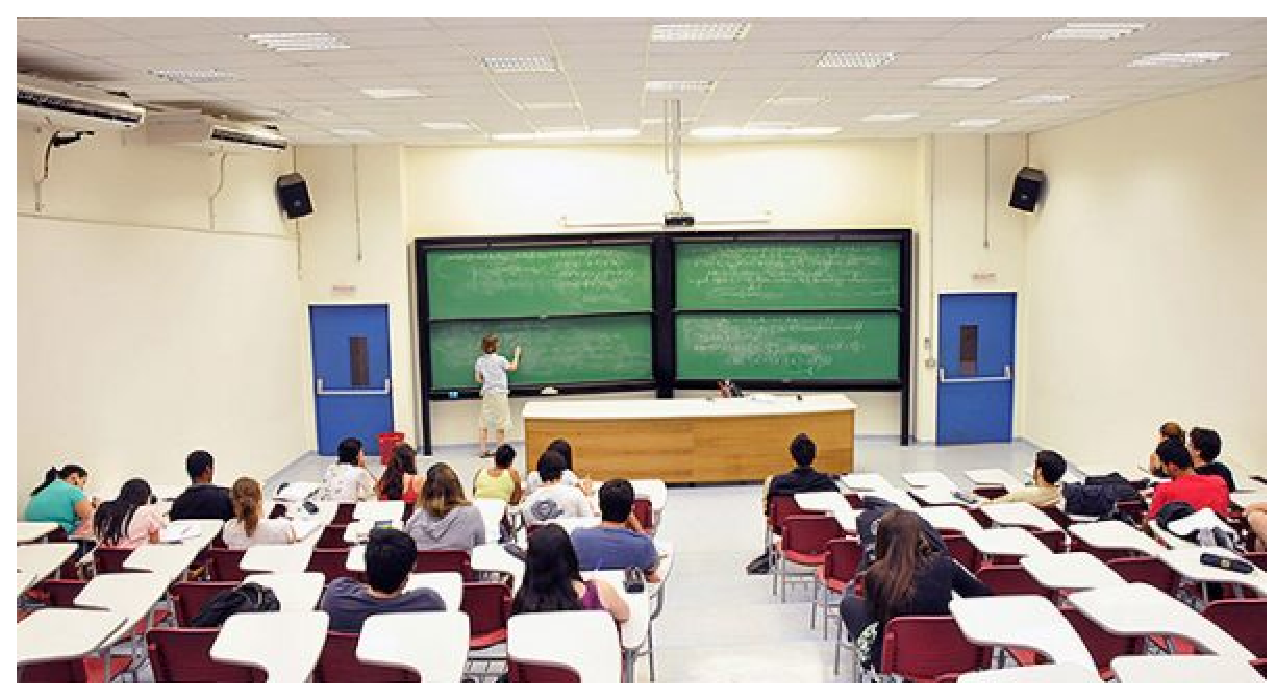
\includegraphics[keepaspectratio=true,scale=0.7]{figuras/unicamp.eps}
 	\caption{Sala de Aula na Unicamp}
 	\label{fig02242}
\end{figure}

\section{Materiais}
O desenvolvimento da construção de um edifício passa por várias etapas. Assim, explicitamos, neste estudo, os materiais utilizados nas etapas gerais de uma obra, levando em conta que elas podem acontecer simultaneamente. Sendo essas: fundações, estruturas/superestruturas, alvenaria, cobertura, acabamentos e revestimentos, esquadrias, pinturas e texturas.

Conforme AZEREDO (1997, pg. 29), fundações, “são os elementos estruturais destinados a transmitir ao terreno as cargas de uma estrutura”. DELILABERA (2011) diz que “a escolha de um sistema de fundações depende de muitas variáveis envolvidas, como: a intensidade dos esforços solicitantes nas fundações [...] a topografia do terreno [...] o custo das fundações, o perfil geotécnico do terreno”. A solução que pode diminuir os impactos ambientais causados pelo uso de concreto seria o uso de concreto de alto desempenho (CAD). Segundo SILVA (2010, pg. 1), “grandes vantagens econômicas e estruturais são obtidas com a utilização do CAD, tais como: redução das seções dos elementos de concreto (pilares), baixa porosidade, baixa permeabilidade, elevada resistência ao desgaste e menor tempo e custo de manutenção”. Levando em conta essas e outras vantagens constata-se que os concretos de alto desempenho são mais sustentáveis que os concretos de resistência usual.

A Superestrutura é um elemento de uma estrutura que se projeta acima da linha de base. No caso de um edifício, representa geralmente a parte do edifício situado acima do solo. Essa estrutura é formada por pilares, vigas, lajes, dentre outros componentes estruturais. Atualmente na construção civil o material predominantemente usado para estruturas é o concreto armado; outras opções são: aço, madeira e compósitos. Priorizando sempre os requisitos de aspecto sustentável do projeto, a melhor alternativa é o uso de estruturas metálicas uma vez que de acordo com ZAPAROLLI(2014):

\begin{citacao}
Estruturas de aço foram consideradas mais amigáveis ao meio ambiente do que as de concreto, madeira ou as de compósito. Isso é resultado da união de dois fatores, o peso relativamente baixo do aço e a facilidade de reaproveitamento do material empregado, uma vez que o aço pode ser reciclado infinitamente.
\end{citacao}


De acordo com CAMPOS: “A vedação por meio de blocos pré-moldados reduz o tempo de execução da obra, propicia maior controle de qualidade e é mais sustentável do que o processo convencional”. (2012, pg. 56) Atualmente, já são produzidos os chamados concretos ecológicos onde é possível substituir até 70\%de areia natural e 100\% de pedra por materiais reaproveitados. É uma opção barata e sustentável para a confecção desses blocos. Os materiais são resultantes da construção ou demolição de edificações e constituem grande volume do resíduo das cidades.

Para a cobertura, uma alternativa moderna e econômica são as lajes nervuradas. Podem ser feitas com concreto ecológico e sua forma geométrica reduz o consumo de aço e concreto em até 30\%, diminuído também o peso total da estrutura.

Os materiais comumente utilizados para esquadrias são: madeira, alumínio, aço e sintéticas. As esquadrias sintéticas de PVC mostram uma gama de vantagens em sua aplicação como: excelente desempenho térmico e acústico, leveza, fácil manutenção, alta resistência e durabilidade, grande estabilidade dimensional e alto índice de vedação e estanqueidade.

Para a pintura e textura serão utilizadas tintas ecológicas feitas a partir de diferentes matérias-primas naturais que não possuem solventes e metais pesados encontrados em pigmentos sintéticos. “É um material atóxico e inodoro, resistente às intempéries, de longa durabilidade, não trinca, não desbota, não descasca e quando descartado na natureza se reintegra sem impactar negativamente”. SOUZA (2011)

Com o recente senso de responsabilidade ecológica e a aplicação dos conceitos de sustentabilidade na construção civil, diversos materiais estão sendo desenvolvidos buscando ser mais eficientes e menos agressivos ao ambiente. No entanto, poucas opções estão disponíveis no mercado ou são produzidos em larga escala, o que torna esses materiais inviáveis ao projeto. Dessa maneira em alguns casos, ainda que existam soluções mais tecnológicas e avançadas, foi necessário se ater a materiais que favorecem disponibilidade, custo e fácil manuseio.

\chapter[Smart Grid]{Smart Grid}

O desperdício energético é uma realidade na FGA. A Faculdade do Gama muitas vezes ultrapassa o limite estabelecido pela concessionária (Companhia Energética de Brasília).

Pode-se abordar diversos pontos quanto à desperdício energético na FGA. A estrutura dos prédios, por exemplo, dificulta a entrada de luminosidade no local, fazendo com que as lâmpadas fiquem acesas durante todo o dia, mesmo sem aulas no local. Outro exemplo são os laboratórios de informática: diversos computadores ficam ligados à tomada durante todo o dia, ainda que não utilizados durante todo o tempo. Existem, ainda, outros exemplos de desperdício energético que serão abordados durante o desenvolvimento do projeto.

Com o objetivo de mitigar os problemas de desperdício energético apresenta-se o Smart Grid: um sistema inteligente de integração entre fontes de produção energética. Essa solução que pode ser divida em duas partes: a primeira remete à geração monitorada de energia, onde o sistema monitora o quanto de energia está sendo produzida e consumida, e armazena esses dados em um banco para futuras análises.(MEDEIROS, William) A segunda parte é definida como um sistema que monitora em tempo real, através de uma rede, problemas que eventualmente podem ocorrer no sistema (como os exemplos de desperdício de energia, cabeamentos com defeitos etc) isolando-os e restaurando o resto do sistema para continuar a sua operação.(FRACARI, Fabiano)

A proposta do projeto é criar um sistema automatizado para o funcionamento das duas etapas do Smart Grid. Utilizaremos um sistema de geração de energia através de fontes renováveis, e essa geração será controlada pelo sistema Smart Grid que guardará os dados de geração/consumo diários, para análise de Gestão e Eficiência Energética.

Esse armazenamento de dados automático é uma das vantagens do sistema, pois diminui consideravelmente a possibilidade de falhas e ainda oferece um planejamento mais eficiente na produção e na distribuição de energia para o Prédio. Além disso, o sistema apresenta uma confiabilidade e uma flexibilidade da rede além do sistema da rede elétrica comum por se tratar de um sistema automático e permitindo que mudanças e/ou reparos possam ser implantados em pontos específicos de acordo com a necessidade sem muito prejuízo ao sistema como um todo(MEDEIROS, William). O sistema também colabora com o desenvolvimento sustentável ao evitar desperdícios e ao ter sua excelente aplicação a fontes renováveis.

Uma desvantagem que iremos analisar é em relação ao custo benefício da implantação deste sistema, que será mais estudado e orçamentado futuramente.Geralmente o sistema é aplicado à redes que interligam uma cidade inteira. Na Europa é crescente o número de implantação de redes inteligentes pois a União Europeia fixou como meta 80\% de medidores inteligentes aplicados à rede até 2020. Já no Brasil o sistema não é aplicado em cidades, mas foi redimensionado para projetos menores. O nosso objetivo é redimensionar o Smart Grid para o Novo Prédio da FGA e fazer um levantamento de custo/benefício da instalação e execução do mesmo.

Uma das características das redes inteligentes (Smart Grid) é o bidirecionamento do fluxo de energia, sendo este não somente radial, partindo das grandes usinas geradoras para os centros consumidores, mas sim, tendo gerações distribuídas em várias partes do sistema, fazendo com que o fluxo não tenha uma só direção. Essa geração distribuída é caracterizada pela instalação de geradores de pequeno porte, normalmente, a partir de fontes renováveis ou mesmo utilizando combustíveis fósseis, localizados próximo aos centros de consumo de energia elétrica. (ANEEL, 2016b)

Com relação a isso, o projeto Prédio Sustentável e Inteligente aplicará o uso da geração distribuída, sendo essa geração oriunda de placas solares fotovoltaica.
A energia fotovoltaica pode ser incorporada em todo território brasileiro, devido às elevadas taxas de irradiação solar em todas as regiões. No Brasil, as regiões Nordeste e Centro-Oeste são as que possuem o maior potencial de aproveitamento de energia solar. Porém as outras regiões apresentam também ótimas irradiações, como por exemplo, a região Sul, que apresenta a pior irradiação nacional e ainda assim é melhor que a irradiação existente em países europeus, nos quais a modalidade fotovoltaica é largamente empregada. (IDEAL, 2015)

O efeito fotovoltaico é resultado da interação da luz com os materiais semicondutores (o mais usado é o silício, pois tem em grande quantidade na natureza) de uma célula fotovoltaica. No interior desta, tal efeito é o responsável pela transformação de energia solar em energia elétrica. A luz solar é composta por fótons que quando incididos no material semicondutor parte deles são absorvidos, excitando os elétrons do material, gerando assim um fluxo de elétrons (corrente). (IDEAL, 2015)

A geração de energia elétrica a partir de placas fotovoltaica é um método bastante difundido atualmente e vem crescendo constantemente. As células solares captam a radiação do sol e através dos fótons geram corrente contínua. Essa corrente passa por um inversor para que seja convertida em corrente alternada com as características da rede (senoidal e frequência de 60Hz). Após passar pelo inversor a eletricidade poderá ser usada para o consumo. Caso a geração exceda o consumo, o restante é inserido na rede e caso o consumo seja maior que a geração solar o restante da energia consumida é oriunda da rede elétrica. (AMERICA DO SOL, 2016)

A instalação do sistema para gerar esse tipo de energia não apresenta grandes complicações, necessitando apenas de uma grande área disponível sem sombras, sendo que seu tamanho dependerá da quantidade de placas necessárias para gerar a energia consumida pelo local a ser instalado. No caso de minigeração (potência instalada de até 75KW) o local mais usado é o telhado, pois apresenta uma grande área isenta de sombras e que não seria usada para outro fim.

A respeito dos documentos regulatórios, no Brasil, existe a Resolução Normativa 428/2012 da ANEEL que foi alterada pela Resolução Normativa 687/2015 da ANEEL. Esta resolução possui conceitos acerca de mini e microgeração e tem como objetivos reduzir os custos e tempo para a conexão da micro e minigeração, compatibilizar o sistema de compensação de energia elétrica com as condições gerais de fornecimento e melhorar as informações na fatura.

Existe também o Módulo 3 do PRODIST (Procedimentos de Distribuição), que estabelece as condições de acesso, compreendendo a conexão e o uso ao sistema de distribuição e define os critérios técnicos e operacionais, os requisitos de projeto, as informações, os dados e a implementação da conexão, aplicado aos novos acessantes bem como aos existentes. (ANEEL, 2016a)

De modo a cumprir um dos requisitos do projeto que é o prédio ser sustentável, será instalado uma mini-usina solar fotovoltaica no telhado do prédio, sendo que sua potência instalada ainda será definida na realização do projeto da mini-usina bem como outros parâmetros necessários, como quantidade de placas, modelo das placas, tipo de inversor, arranjo das placas, distanciamento entre as mesmas, orientações e angulação, dentre outras coisas.

A mesma terá que possuir uma potência instalada capaz de suprir toda a demanda de energia consumida no prédio de modo que a parcela de energia consumida seja zerada na fatura. Como a faculdade faz parte dos consumidores do grupo A (alta tensão), a mesma ainda pagará a parcela de demanda contratada para a distribuidora.

A manutenção adequada dos painéis solares evita a deterioração, reduz custos com substituição de peças e aumenta sua vida útil. Na maioria das vezes, a chuva fará a maior parte do serviço, pois telhados no Brasil possuem 15 graus ou mais de inclinação, facilitando que a água da chuva escorra sobre o painel e assim levando a poeira embora. Porém, caso seja necessário (devido a sujeiras maiores como fezes de animais) sua manutenção é bastante simples, basta fazer uma pequena limpeza seguindo os seguintes passos: 1)Desligar o sistema fotovoltaico; 2)Usar uma escova macia de boa qualidade ou um rodo com uma lâmina de plástico em um lado e um pano amarrado, juntamente com uma longa extensão(Evitar usar objetos metálicos ou produtos abrasivos) ;3) Usar uma mangueira com um bico adequado para permitir que o jato de água chegue até os painéis (Não aplicar pressão e não bater ele nos painéis). A melhor hora para manutenção é em um dia nublado, no início da manhã ou à noite (se o sol estiver forte a água pode evaporar rapidamente dificultando a limpeza). Outro bom horário é ao amanhecer, pois o orvalho noturno poderá amolecer a sujeira, facilitando o processo de limpeza e economizando água e energia.
Tendo em vista a necessidade de uma constante manutenção nas placas o projeto também irá desenvolver um sistema de manutenção automático onde o mesmo por meio de sistemas eletrônicos e softwares irá detectar o problema e resolvê-lo, caso seja necessário uma manutenção com mão de obra o sistema irá informar.Esse sistema está em discussão para melhor atender a universidade e estará mais compacto com decorrer do desenvolvimento do projeto.

O payback do investimento ainda será calculado, mas sabe-se que a instalação se paga em torno de 6 à 9 anos e que os painéis têm uma vida útil mínima de 25 anos (se bem mantidos) e que os inversores têm uma vida útil de 10 anos, por tanto, a instalação de uma usina solar fotovoltaica é rentável.

Tendo em vista um sistema reserva de energia caso algum problemas ocorra com a fonte de energia principal foi discutido a importância de um sistema que supra essa demanda energética até que o inconveniente seja resolvido foi proposto ao projeto um gerador que utiliza um combustível sustentável que pode ser produzido na própria universidade.

\section{Gerador movido a biodisel}

A queima de combustíveis fósseis gera poluição, sobretudo poluição atmosférica, devida à emissão desses poluentes por meio da queima de geradores de energia, como também de automóveis (VALENTE, 2007). Dentre esses poluentes se destacam material particulado (MP), hidrocarbonetos e os chamados gases estufa (dióxido de carbono, metano, óxido nitroso, clorofluorcarbono CFCs) podendo causar sérios impactos ambientais, sociais e também econômicos (BRAGA, 2005).

Em contrapartida, busca-se o desenvolvimento e aperfeiçoamento de biocombustíveis, como o biodiesel, como pode ser visto na Figura 01, que a produção do biodiesel vem crescendo (ANP, 2016), por ser uma fonte de energia limpa e renovável, polui menos que o petróleo, podendo reduzir a dependência brasileira das importações deste insumo, além de proporcionar vantagens econômicas, criando milhares de empregos, principalmente na agricultura familiar e nas regiões mais pobres do Brasil (JARDINE, 2009)
\pagebreak
 \begin{figure}[!h]
 	\centering
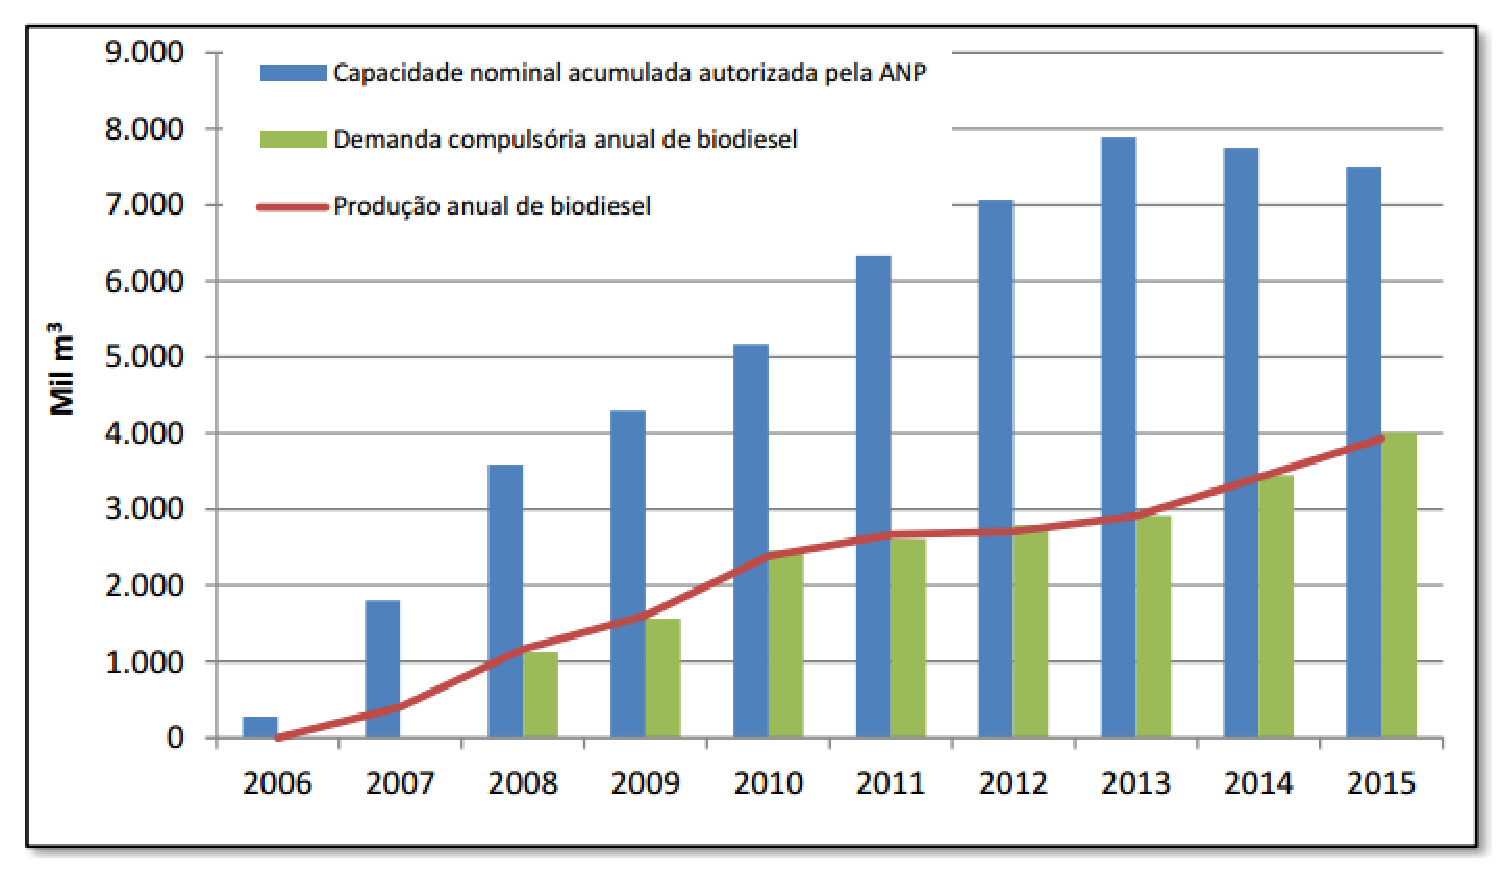
\includegraphics[keepaspectratio=true,scale=0.5]{figuras/producao.eps}
 	\caption{Evolução anual da produção, da demanda compulsória e da capacidade nominal autorizada pela ANP no país}
 	\label{fig02242}
\end{figure}

O biodiesel tem uma característica vantajosa, pois é possível substituir o óleo diesel, sem requerer adaptações mecânicas, ao contrário de outros combustíveis limpos, tais quais o gás natural ou biogás e o álcool etílico, portanto, contribui para uma viabilidade técnica (VOLPATO, 2009).

Visando uma sustentabilidade para o novo prédio da Faculdade Gama da Universidade de Brasília (FGA/UnB), propõe-se a instalação de um gerador à biodiesel a fim de suprir uma falta de energia fornecida pelas placas fotovoltaicas e da Companhia Energética de Brasília (CEB), ou até mesmo seu funcionamento em tempo integral; e uma integração com o Projeto BioGama realizado na FGA/UnB.

Sabendo que se forem adotadas certas estratégias, como o crédito de carbono, a utilização do gerador não só em caso de emergência, como também em horário de pico, o gerador à 100\% biodiesel (B100) apresenta resultados atraentes economicamente.
\section{Reaproveitamento de Recursos Hídricos}

Reaproveitamento da Água está em crescente expansão na construção dos prédios atuais a análise da viabilidade do reaproveitamento da água utilizada e a crise hídrica no Distrito Federal vem para aprofundar essas discussões .Como o prédio será sustentável e localizado em uma das regiões administrativas do DF ,nada mais importante do que avaliar a implantação desse sistema no novo prédio.

Os sistemas de reaproveitamento ou de reuso que foi proposto é o de captação da água da chuva por meio de calhas que levam a tanques de tratamento, e também pela reutilização da água utilizada em lavatórios , ralos dos chuveiros, águas de ar condicionado, excluindo as águas utilizadas em descargas dos banheiro ,pois estamos falando do reaproveitamento de águas cinzas ,aquelas as quais pode se fazer um tratamento simplificado.As águas adquiridas desse processo poderão ser utilizadas em irrigação de jardins ,descargas de banheiros ,lavagem e automóveis de funcionários e muito mais ,com isso a FGA iria além de economizar recursos hídricos promover uma educação para economizar água mostrando a cidade do gama como é possível reaproveitar a água.

\chapter[Controle de Acesso]{Controle de Acesso}
A respeito do nosso escopo interno, ficamos responsáveis pela parte de controle de acesso ao prédio e a faculdade, e para isso dividimos nossos componentes em três principais grupos, que são, controle de acesso nas salas e laboratórios, controle de acesso ao estacionamento privativo da faculdade e controle de frequência nas aulas. Em todos esses casos, foram pensadas soluções práticas, acessíveis, viáveis e criativas, e dentre todas as possibilidades, foi escolhido o sistema RFIG ( Identificação de Rádio Frequência), que integrará todo o sistema de acesso dentro da universidade.

 Um dos grandes problemas que existe da FGA é o estacionamento precário e sem segurança que disponibilizam para os alunos e funcionários, e pensando justamente nisso, seria viável um estacionamento seguro com controle de acesso. O controle de acesso seria composto por cancelas, interfones, sistema RFID de identificação e câmeras, todos trabalhando de forma integrada com a guarita de vigilantes dentro do prédio inteligente da faculdade, com intuito de garantir a integridade física e material de quem utiliza o campus. O sistema funciona da seguinte forma: o motorista irá chegar na entrada principal do campus, composta apenas pela cancela e um painel de controle, onde irá passar seu cartão de acesso RFID, e este através de um banco de dados irá fazer o reconhecimento do aluno e liberar sua entrada, lembrando que o mesmo processo será feito na saída dos carros. Caso o motorista seja um visitante, ele será instruído via interfone a dar dados pessoais para o vigilante, na guarita, assim tais dados serão registrados em um banco de dados para entrada e saída do visitante.

O sistema foi desenvolvido levando em conta que as pessoas podem perder ou esquecer seu cartão de acesso em algum dos dias letivos, se tal eventualidade ocorrer ao aluno, professor ou servidor será instruído a dar sua matrícula ou dados pessoais ter o rosto fotografado e assim terá sua entrada liberada, e para sair será o mesmo processo. As vantagens desse processo todo está na segurança e em alguns casos prover validade jurídica, comprovando a presença ou não do veículo no estacionamento, e por outro lado, as desvantagens estão na necessidade na mudança de cultura dos usuários, homologação da ANATEL para que o sistema funcione e lentidão nos horários de pico.

Outra parte importante que faz parte do nosso escopo, é o controle de acesso nas salas e laboratórios, que será feito com um dispositivo conectado a fechadura eletrônica em cada porta. A ideia principal da solução é manter determinadas salas trancadas na maior parte do tempo para maior segurança e controle no uso dos bens materiais nela presentes e, registrar a presença de um responsável pela sala no instante de entrada na sala.

Com isso, haverá a necessidade de reservar uma sala/ambiente especial, com equipamentos simples, para ser utilizado como sala de estudos do campus, já que grande parte das salas estariam trancadas nos períodos em que não houvessem aulas.

A princípio seria necessário registrar os perfis dos usuários das salas num banco de dados, tais perfis seriam de aluno, professor e funcionário. Cada perfil existente possuirá permissões diferentes em relação ao acesso às salas e laboratórios, um professor ou funcionário registrado tem permissão para abrir qualquer sala de aula ou laboratório, que estará sob sua responsabilidade desde o momento da entrada até a saída da sala, já um aluno registrado tem permissão para abrir qualquer sala de estudo que possua apenas equipamentos simples, caso o aluno queira entrar numa sala que disponha de equipamentos de alto valor, será necessária a presença de um professor ou funcionário nesta sala. É importante ressaltar que um responsável por uma sala/laboratório teria a função de alertar à secretaria qualquer irregularidade detectada no ambiente, caso contrário, ele seria o responsável por tais irregularidades ocorridas no período registrado.

As vantagens desse sistema estão na dificuldade de fraude no sistema, baixo custo, e maior zelo pelos bens da faculdade, e por outro lado, a desvantagem seria a intimidação dos alunos em se responsabilizar pela sala, em alguns casos.
E como última forma de controle de acesso, temos o controle de frequência nas aulas, que será implementado por meio de um aparelho portátil leitor RFID com display e teclado alfanumérico, como o mostrado abaixo.

\begin{figure}[!h]
 \centering	\includegraphics[keepaspectratio=true,scale=0.5]{figuras/freq.eps}
 \label{fig022433}
 \caption{Imagem ilustrativa do aparelho portátil de frequência}
\end{figure}
\pagebreak

O sistema entra em funcionamento quando o professor entrar na sala, ou até mesmo antes de entrar, ele vai ligar o aparelho, que será conectado à rede WiFi da UnB, digitar o código e turma da matéria e baixar os dados dos alunos cadastrados naquela disciplina. Com os dados já baixados, o aparelho seria passado de mesa em mesa, e cada aluno passaria seu cartão para marcar presença na aula, e com tudo isso, o professor estaria ministrando sua aula, sem perda de tempo. A possibilidade de burlar o cartão não seria bem sucedida pelo fato de todo cartão gerar um token único, impossibilitando a clonagem de cartões, e mesmo existindo a possibilidade de amigos deixarem seu cartão um com outro, geraria uma série de problemas dentro da faculdade. Um dos problemas que poderia ocorrer seria a possibilidade de queda no sinal de WiFi, contudo o aparelho tem o artifício da memória interna para esses casos, e assim que a conexão reativar, os dados são enviados automaticamente. Outro obstáculos estaria nos alunos esquecerem de levar a carteirinha, mas para essa situação bastaria conversar como o professor e resolver sem muitos problemas

Então, as vantagens desse sistema está na praticidade, dificuldades para fraudar e custos baixos, já a desvantagem maior está no possível esquecimento do cartão e em um possível processo longo para conseguir um cartão novo, em casos de quebra ou roubo/furto.

Diante de tudo apresentado, é notável que seria necessário apenas um documento de identificação para o acesso em todos os casos citados acima, que seria a própria carteirinha que já usamos normalmente na faculdade. Outra coisa em comum, é que também foram pensados os sistemas de biometria e análise de código de barras, entretanto eles foram descartados por conta do custo alto e dá maior possibilidade de falha no sistema por conta de fatores externos, especialmente o sistema de biometria, que de acordo com o estudo: Advantages And Disadvantages Of Biometrics da UK Essays, gera uma falha na impressão digital de algumas pessoas e decaimento da performance do dispositivo.



\chapter[Instrumentação e Controle]{Instrumentação e Controle}
\section{Introdução}
A automação é inerente a um prédio inteligente, porém deve ser implantada de forma que a usabilidade seja fator prevalecente no projeto. Para automação das salas de aula e laboratório essa etapa foi dividida em subáreas, de modo a problematizá-las e solucioná-las. São elas: ambientação da sala, painéis de controle, sensores, digitalização  e integração dos equipamentos para aula, status da sala e monitoramento do prédio.

\section{Ambientação da Sala}
\subsection{Iluminação}
Atualmente, a Faculdade do Gama da Universidade de Brasília tem em sua maioria aulas expositivas, estas realizadas com auxílio de slides, quadros brancos e quadros negros.

Para cada sala existem dois pontos principais de iluminação, a iluminação para os alunos presente em toda a sala e a iluminação do quadro. Sendo necessário ir durante a aula apagar ou ligar determinada lâmpada, pois a luz que ultrapassa as janelas e reflete no quadro dificulta a leitura do que está presente no mesmo. Além disso, se tratam de lâmpadas fosforescentes tubulares, que possuem uma vida útil menor, possuem um preço muito elevado considerando as variáveis de consumo de energia elétrica e a vida útil.

Visando resolver problemas com a quantidade de luminosidade para cada momento de uma aula expositiva, variando entre escura para apresentação de slides e clara para ministração do conteúdo da disciplina, para a praticidade e pouca manutenção fora escolhida uma lâmpada inteligente: a lâmpada Alba.
Uma lâmpada que possui um sensor que se adapta às condições luminosas do usuário, produzindo uma iluminação customizada para cada situação, pois é sensível às variações da luz solar com o passar do dia. Ela possui. também, um sensor de movimento, o que a liga quando detectado algum movimento, característica útil para fatores de segurança.

Sua emissão de luz pode variar entre branco e amarelo, que dão sensações diferentes ao usuário. Sendo branco necessária para aumentar a concentração e amarela para dar sensações de calor. Essa configuração é alterada adaptando-se ao ambiente que a lâmpada está.

A lâmpada inteligente Alba foi idealizada para não precisar de aplicativos ou controles para ser modificada, tornando-a totalmente adaptável ao cliente. Não obstante, o fabricante disponibiliza um aplicativo para controlar o dispositivo, como explicado em sua página na web: “Apesar de termos lutado para minimizar a necessidade de interação do usuário, o stack lighting app permite a você customizar diversos dos recursos que vêm instalados, esses incluem:

\begin{itemize}
\item Mudando a temperatura da cor de 2700k (branco amarelado) para 6500k (branco azulado)
\item Mudar	o nível da intensidade da luz máxima e mínima.
\item Agendar mudanças de cor, temperatura e intensidade.
\item Agendar tempo de acordar.” \cite{light2017}
\end{itemize}

Essa possibilidade de configuração predeterminada a torna diferente de um dimmer comum, pois poderia ser estabelecida antes de cada aula.

Para utilizá-la nas salas, seria-se capaz de configurar, por meio do aplicativo, para acender no horário que começam as aulas e apagar quando acabam as aulas, ou para acender quando detectar um movimento. Dessa forma, não seria necessário ligá-las, uma a uma, manualmente. Também seria possível determinar a quantidade de luz cada uma deve emitir.

Além disso, para a integração da sala será acrescentado o aplicativo de controle da lâmpada na mesa inteligente que será utilizada pelo professor e será descrita posteriormente.

\subsection{Persianas Inteligentes}

Em virtude da localização do campus da Faculdade do Gama, existe um problema que não pode ser totalmente solucionado: a poeira. Esta inibe a abertura das janelas, para que ela não entre nas salas com muita intensidade, o que prejudica a circulação de ar no ambiente. Além disso, em alguns horários a luz do sol entra pelas janelas e reflete nos quadros, o que dificulta a leitura e/ou a visualização de slides. Para resolver estes problemas, serão utilizadas persianas automatizadas em cada sala de aula.

Estas persianas são feitas de um material resistente, e podem serão instaladas na parte interna das salas. O espaçamento entre cada haste pode ser regulado, para limitar a quantidade de luz natural que entra na sala. Além disso, a fabricação das persianas impede a entrada de poeira, reduzindo os problemas que ela causa, e quando totalmente fechadas, fornecem isolamento acústico, o que pode ser útil durante o período entre as aulas, por exemplo.

As persianas são controladas a partir de um mesmo ponto, simplificando e diminuindo a movimentação para abrí-las ou fechá-las dentro da sala.

A marca Somfy fornece persianas que podem ser controladas através de um tablet, assim pode-se centraliza a todas as funções num mesmo aparelho e programa os horários para abrir ou fechar \cite{somfy2017}. Essas funcionalidades poderiam ser transferidas para a mesa inteligente.

\subsection{Sistema de Som}
Um sistema de som, com alto-falantes em pontos estratégicos das salas de aula e o uso de um microfone para o professor estará presente em cada sala do prédio. Este sistema visa melhorar a comunicação entre professores, diminuindo o esforço de uso da voz, e os alunos, amplificando a fala do professor e a tornando mais clara em todos os locais da sala.

\subsection{Climatização}
O fechamento das janelas para evitar a entrada de poeira dificulta a circulação de ar nas salas, aumentando a temperatura nos horários mais quentes do dia. Além disso, o Distrito Federal enfrenta períodos com baixa umidade do ar, causando mal estar nas pessoas que convivem na faculdade. Para resolver este problema serão utilizados ares-condicionados nas salas.

Condicionamento de ar consiste no tratamento do ar em locais fechados. Isso regula e qualifica o ar presente em determinado ambiente. Tratando as condições de temperatura, limpeza, umidade e movimento. Um ar condicionado é responsável por aquecer, umidificar, filtrar, renovar e refrigerar o ar.

Para configuração do ar condicionado, será utilizado um termopar para aferir a temperatura do ambiente, com um display para mostrar o valor em graus Celsius. O termopar estará conectado a uma função lógica programável em que ao chegar a determinado grau, o termostato do próprio ar condicionado deve se configurar em determinado grau de resfriamento. Isso fará com que o movimento e a constante configuração diminuam, visto que só será necessário controlar o grau quando se desejar um valor diferente do anteriormente configurado. Esse valor será determinado para que a sala fique climatizada adequadamente, com um clima ameno.

\section{Painéis de Controle}
\subsection{Controles embutidos na mesa inteligente}
Após automatizadas as funcionalidades da sala de aula, o meio utilizado para controlá-las de maneira interconectada será uma mesa inteligente. Dessa forma muitos dos empecilhos vistos cotidianamente no campus (dificuldade ou demora para uso do projetor e controle da ambientação da sala, já citado anteriormente) poderão ser facilmente manejados.

\subsection{Controle geral para a sala}
É importante que haja um controle externo à mesa inteligente para acesso dos funcionários e outras eventualidades. Portanto, algumas das funcionalidades, principalmente aquelas que dizem respeito a ambientação da sala, terão este controle adicional. Será o caso da persiana e do ar-condicionado, que possuirão controle remoto.

\subsection{Sala de controle}
O prédio sustentável irá dispor de uma vasta gama de sensores e equipamentos que irão fornecer feedback em tempo real sobre todas as suas áreas. Estes dispositivos podem enviar informações sobre o funcionamento de equipamentos eletrônicos, a pressão em tubulações hidráulicas e até sobre a integridade do concreto da edificação.

O processamento destes dados, além do controle de alguns dispositivos que executam as operações do prédio, será concentrado em uma sala de central de controle onde todos os dispositivos são conectados, o que caracteriza um sistema de automação centralizado \cite{dias2004}.

Os sistemas centralizados, como o nome sugere, são aqueles que dispõem de uma unidade central de controle pela qual todos os dispositivos da instalação são conectados, tanto para o recebimento dos sinais dos sensores, quanto para, após o processamento dos sinais, enviar os comandos e ajustes aos dispositivos receptores para que executem as operações.

\section{Sensores}
Em qualquer automação predial um dos componentes mais utilizados é o sensor. Sua função, responder a estímulos físicos e mensurá-los analogicamente, obviamente é de suma importância neste tipo de projeto. Os sensores utilizados nas etapas referidas na automação, serão brevemente citados a seguir.

\subsection{Termopar}
O termopar é um sensor de temperatura simples, de baixo custo, e de fácil funcionamento, utilizado no condicionamento de ar para aferir a temperatura do ambiente. É um dispositivo com dois condutores metálicos diferentes unidos em uma extremidade, expostas a variação de temperatura, captando-o.

\subsection{Termostato}
O fototransistor é um tipo de sensor de luz utilizado pela lâmpada Alba. Ele possui duas junções semicondutoras que variam sua resistência elétrica em função da intensidade da luz.

\subsection{Fototransistores}
O sensor de movimento utiliza da tecnologia infravermelho e fototransistores para captar a informação como um receptor transmissor. Eles atuam na faixa óptica da radiação térmica, com isso responde o calor entre o sensor e o objeto analisado. O princípio da detecção de movimento pelo calor é fundado na teoria da emissão de radiação eletromagnética.

\subsection{Sensor de movimento}
O sensor de movimento utiliza da tecnologia infravermelho e fototransistores para captar a informação como um receptor transmissor. Eles atuam na faixa óptica da radiação térmica, com isso responde o calor entre o sensor e o objeto analisado. O princípio da detecção de movimento pelo calor é fundado na teoria da emissão de radiação eletromagnética.

\subsection{Sensor de calor}
É um transdutor que gera um sinal elétrico proporcional ao fluxo de calor aplicado em sua superfície. Para a aplicação em edifícios, sua maior utilização é para a qualidade do isolamento térmico. Para o caso do novo prédio da Faculdade do Gama, será utilizado para analisar a possível presença de calor provinda de fogo ao arredores do prédio. Será conectado a uma função lógica programável para que quando detectar determinado valor em graus Celsius, acione a função contra incêndio.

\section{Digitalização e Integração de Equipamentos para Aula}
\subsection{Mesa inteligente}
Nas últimas décadas pesquisas e projetos de dispositivos eletrônicos multi-toque em formato de mesa vêm surgindo. Este tipo de tecnologia já pode ser encontrada em alguns museus e lojas de varejo \cite{horn2008}. Seguindo esta tendência, somada ao fato de que o uso de tecnologia no ambiente educacional tem sido cada vez mais incentivado, e se tornou comum aos estudantes \cite{bulman2015}, uma mesa inteligente e interativa estará presente em cada sala de aula, para auxiliar o professor durante as aulas.

Este dispositivo consiste em uma tela sensível ao toque, em formato de mesa, que permitirá que o professor controle os diversos dispositivos presentes na sala, como projetores, quadros, sistema de som e até a climatização e iluminação do ambiente.

Atualmente, no mercado, existem algumas soluções que se adequam ao contexto deste projeto. As características de cada dispositivo varia de um fabricante para outro, como por exemplo o tamanho da tela sensível ao toque, sendo encontradas usualmente telas de 32 a 65 polegadas, ou a presença de tecnologias de reconhecimento de objetos colocados sobre sua superfície.

As mesas interativas possuem suporte para diferentes sistemas operacionais, como Windows, Linux, MacOs X, e até Android, o que permite a fácil integração com outros dispositivos como projetores e roteadores de internet. Isto pode possibilitar ao professor o acesso a materiais disponíveis online durante a aula, facilidade de exibição de apresentações em slides entre outras inúmeras possibilidades de uso, além de possuir um controle centralizado de todas as funções automatizadas presentes na sala de aula.

\subsection{Quadro interativo}
	Estudos apontam que a utilização de quadros interativos durante aulas expositivas pode ser uma prática positiva, pois permite que elementos computacionais sejam integrados ao ambiente sem “quebrar” a comunicação \cite{mech2007} \cite{gerard1999}. Por este motivo, esta tecnologia será  utilizada nas salas de aula do prédio.

Atualmente existem diversos fabricantes de quadros interativos, com diferentes tamanhos e funcionalidades, incluindo até, em alguns casos, suites de softwares específicos para aquele determinado produto. Os dispositivos possuem diversas opções de conectividade, possibilitando a interação com computadores pessoais, dispositivos mobile e até mesmo com a mesa inteligente do professor.

É importante ressaltar que a utilização de quadros interativos não irá excluir os quadros convencionais das salas de aula, permitindo ao professor escolher qual ferramenta será mais adequada ao seu contexto.

\subsection{Sistema de projetores}
A sala de aula terá também um sistema de projetores, para possibilitar apresentações de slides, vídeos, apresentação de documentos, textos, páginas da web entre outras mídias. Esta ferramenta, somada aos outros dispositivos interativos disponíveis na sala de aula, irão fornecer uma vasta gama de opções para auxiliar o professor durante as aulas, de acordo com cada contexto.

\section{Status da Sala}
\subsection{Painel informativo}
Com o objetivo de manter sempre disponíveis informações sobre cada sala de aula, serão instalados painéis informativos na entrada de cada uma delas. Estes painéis consistem em telas LCD LED, que irão exibir informações sobre cada sala de aula, como sua capacidade máxima, quando, em quais horários e por quem a sala será utilizada, avisos informativos, entre outras.

Estes painéis serão conectados à internet, possibilitando o envio de avisos em tempo real, para informar sobre cancelamentos ou mudança de local das aulas, por exemplo. Além disso, alunos, monitores, professores ou outros interessados poderão reservar as salas em determinados horários por meio do aplicativo da FGA, baseando-se na agenda exibida nos painéis.

\section{Monitoramento do Prédio}
De acordo com a norma NBR 5462 existem basicamente três tipos de manutenção: Corretiva, Sistemática e Condicional \cite{souza2010}.

A Manutenção corretiva é uma política onde o conserto é realizado após a ocorrência do defeito. Este tipo de abordagem gera prejuízos pois o custo aumenta em função da idade do equipamento, além de exigir a parada imprevista de seu funcionamento.

Já a manutenção sistemática é feita de forma preventiva, ocorrendo periodicamente de acordo com critérios estatísticos ou recomendações do fabricante. Esta prática pode implicar em manutenções desnecessárias ou ineficazes, além da possibilidade de introdução de novas avarias durante o processo de montagem e desmontagem do equipamento.

Por fim, a manutenção condicional, também conhecida como manutenção preditiva, consiste em um tipo de manutenção preventiva que, ao invés de ser realizada em intervalos predeterminados, é baseada em informações sobre o estado de degradação do equipamento ou sistema. Esta modalidade de manutenção visa mitigar as desvantagens das práticas descritas anteriormente.

No projeto do prédio sustentável, a manutenção preditiva será peça chave para manter os diversos dispositivos de automação em pleno funcionamento. Em diversas áreas do prédio, sensores com diferentes funções e comportamentos irão enviar dados para uma central de processamento, proporcionando um feedback contínuo sobre o funcionamento de todo o sistema. No caso de uma anormalidade detectada em alguma área do prédio, uma equipe de manutenção será automaticamente designada para analisar e corrigir a falha em potencial.

\chapter[Interfaces e Processamento de Software]{Interfaces e Processamento de Software}

A Engenharia de Software é uma área, dentre as muitas existentes, que abrange  e aborda o conhecimento voltado para
a informática, e a computação. Lida com vários aspectos do desenvolvimento de software, tais como, planejamento,
 desenvolvimento, manutenção e desenvolvimento de sistemas de software, gerência de projetos e outras disciplinas,
 com objetivo de obter organização, qualidade e produtividade \cite{gungor}.

Dentre as habilidades que os engenheiros, em comum, devem possuir, tais como raciocínio lógico e matemático, o Engenheiro de Software deve ter um gosto maior pela inovação e uma capacidade mais alta em atualizar-se continuamente, já que software é uma área que está em constante mudança. Com tais mudanças e surgimento acelerado de novas tecnologias e informações \cite{daneels}, é perfil do profissional, estar sempre disposto a deixar seu ponto de conforto para obtenção de novos conhecimentos. Além de ter um bom entrosamento para trabalhar em equipe e uma visão abrangente do mundo, sociedade
e suas dinâmicas \cite{daneels}.

Esse é um curso relativamente novo e é ministrado em poucas faculdades brasileiras, na Universidade de Brasília (UNB) este curso é ministrado na Faculdade do Gama UnB (FGA) e assim como o curso, a FGA também é nova. Atualmente a faculdade é composta por três prédios:

\begin{itemize}
\item \textbf{Unidade Acadêmica (UAC)}\textbf{:} É onde se encontra a maior parte das salas de aula, bem como o Auditório, a Biblioteca da FGA, alguns laboratórios e os espaços de convivência dos alunos.
\item \textbf{Unidade de Ensino e Docência (UED):} É onde ficam as salas dos professores, coordenadores e a direção do Campus. Também se encontram nesta unidade os principais laboratórios e a Enfermaria.
\item \textbf{Módulo de Serviços e Equipamentos Esportivos (MESP):} É onde se encontra o R.U.(Restaurante Universitário). E tem como anexo uma quadra poliesportiva aberta a todos.
\end{itemize}

Existem também outras estruturas que se encontram fora da área da faculdade, sendo elas:

\begin{itemize}
\item \textbf{Fórum: }Lugar onde se encontram os principais laboratórios de Engenharia de Software e onde são ministradas as aulas de mestrado e especialização.
\item \textbf{Galpão: }Depósito de ferramentas, insumos de construção, peças e outros objetos. Também estão localizados lá os principais laboratórios de Engenharia Automotiva.
\end{itemize}

A lotação do campus da FGA é imprescindível, tendo em vista que o que tem-se como campus hoje é apenas uma parte do projeto final. Todavia, não há o planejamento da diminuição de vagas disponibilizadas para os vestibulares semestralmente.

Com base na lotação da FGA e que não há diminuições de vagas de ingresso na faculdade, é necessária a construção de um novo prédio, para futuramente alocar novas salas de aula e laboratórios. De acordo com o projeto, com o contexto do campus envolvido e com a situação à qual o Brasil se encontra atualmente, deverá ser um prédio sustentável e inteligente para redução de custos e otimização de recursos.

Tratando-se de Software, com a integração das demais engenharias do campus, deve-se compor o novo prédio e o projeto, equipamentos “inteligentes” que identificam falhas, erros no consumo de energia e que sejam sustentáveis, no quesito de funcionamento. Com uso de sensores, saber quando deve ser ligado/desligado.


\section{Aplicativo}

Segundo Reinhard(2007) “Com o crescimento da telefonia móvel, banda larga e redes sem fio, a mobilidade e a computação em múltiplas plataformas e aparelhos tornam-se cada vez mais factíveis” graças a esse crescimento e a mobilidade construiremos um aplicativo idealizado para que os usuários possam gerenciar as informações disponibilizadas pelo Smart Grid sobre o consumo de energia, podendo questionar os responsáveis pelo resultado obtido. Este auxiliará também na identificação de possíveis problemas que o próprio sistema não consegue identificar e consertar, tendo em vista que o usuário poderá relatar sobre as falhas encontradas. Também informará o status de cada sala que compõem o prédio, tais como lotação, agendamento, disponibilidade.

No controle e comunicação entre os usuários do prédio e os responsáveis legais pela gestão do mesmo o aplicativo dará seu devido suporte. Os usuários podem gerenciar as informações disponibilizadas pelo Smart Grid e passar um feedback relacionado à possíveis problemas que o sistema não conseguiu identificar. O software também informará sobre o status de cada sala que compõem o prédio e seus objetos novamente permitindo que os usuários informem problemas aos gestores do prédio.

A equipe de Interfaces e Processamento de Software e a de Smart Grid idealizaram, conjuntamente, a parte do aplicativo responsável por gerenciar as informações disponibilizadas pelo Smart Grid, o qual informará aos usuários sobre o consumo de energia de cada sala e laboratório do prédio. Com tais informações, os usuários poderão ter um controle maior sobre a quantidade de energia gasta no prédio, podendo questionar os responsáveis por tais resultados, caso estejam fora dos parâmetros.

O aplicativo disponibilizará uma ferramenta na qual os usuários poderão relatar sobre problemas identificados no prédio, sendo assim, uma forma mais eficiente para entrar em contato com a coordenação, a qual terá mais rapidez na hora de solicitar reparos. Isso será possível através de um banco de dados que armazenará o código único de cada item da sala de aula e laboratórios, como mesas, cadeiras, quadros inteligentes, projetores, e equipamentos diversos em laboratórios. O usuário do aplicativo, ao perceber algum equipamento ou item da sala de aula danificado, deve entrar com esse código único, na seção de “problemas encontrados”, e o aplicativo notificará os responsáveis pelos reparos.

Além disso, o software também disponibilizará para os usuários o status de cada sala ou laboratório do prédio. Informando a lotação da sala no horário da aula para o usuário poder se localizar rapidamente, horários de limpeza para cada sala e se há disponibilidade de horário para poder utilizá-la. Paralelo a esses recursos o aplicativo possuirá um sistema de reserva de salas para que elas possam ser utilizadas em seus horários livres por monitores, palestrantes, professores e alunos.


		\section{Construção de Software no Smart Grid}

Smart grid é uma infraestrutura de energia elétrica moderna para melhorar a eficiência, a confiabilidade e a segurança, integrando vários tipos de energias alternativas através da automação e modernas tecnologias de comunicação \cite{gunda}. Para realizar todas as tarefas o sistema precisa adquirir, processar, organizar e também disponibilizar os dados coletados, isso é possível adotando um software de supervisão e monitoramento SCADA (Supervisory Control and Data Acquisition). Os Sistemas de Supervisão e Aquisição de Dados são tipos de sistemas que utilizam softwares para monitorar os dispositivos de controle oferecendo qualidade, redução de custos, e alto desempenho. O sistema conta também com uma possível integração com outros sistemas de cálculo como o SPC (Statistic Process Control), OEE (Overall Equipment Effectiveness), entre outros \cite{daneels}.

O software será alimentado com os dados do edifício através da implementação do smart grid sendo que todos esses dados serão repassadas ao aplicativo, meio visual por onde as informações serão repassadas e interpretadas pelos usuários.
Para processar essas informações o software terá uma estrutura similar à apresentada na figura a seguir.
\pagebreak
\begin{figure}[!h]
 \centering	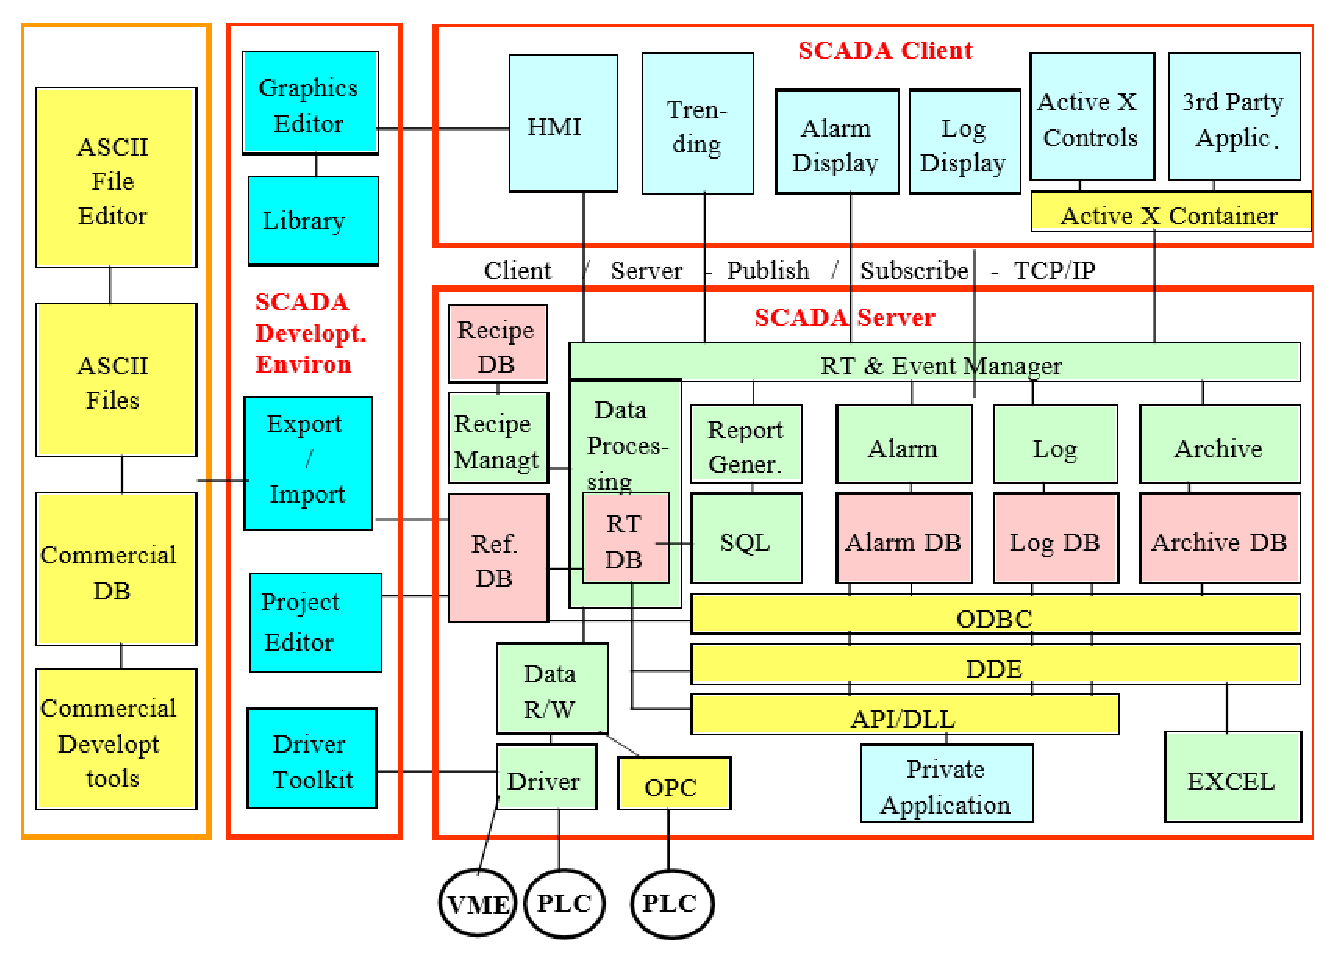
\includegraphics[keepaspectratio=true,scale=0.6]{figuras/sof.eps}
 \caption{Estrutura genérica para software SCADA }
 \label{fig022}
\end{figure}

O sistema pode oferecer consultas a histórico de eventos e também gráficos históricos que são importantes para o monitoramento da real eficiência do prédio. Esse modelo de software de supervisão irá complementar a eficiência esperada do smart grid, integrando os sistemas e oferecendo interfaces gráficas para o usuário.


		\section{Banco de dados do prédio}


Os bancos de dados modernos oferecem os mais variados tipos de serviços, entre eles há a opção de se utilizar armazenamento em nuvem e armazenamento local de dados.

“Computação em nuvem é uma tendência recente de tecnologia cujo objetivo é proporcionar serviços de Tecnologia da Informação (TI) sob demanda com pagamento baseado no uso” Souza, Moreira e Machado(2009). A computação em nuvem “permite o acesso aos dados sem necessidade de instalar softwares, podendo ser acessado de qualquer lugar pela internet” Rosário, Colling e Soares(2015), ela funciona por meio de um hardware físico chamado servidor que disponibiliza seus recursos e até programas em rede, podendo estes serem acessados em qualquer lugar do mundo. Por fim os recursos são utilizados por usuários que armazenam ou consomem dados. Apesar de ser muito mais versátil esse modelo pode apresentar problemas de segurança e de velocidade de acesso a informações já que depende inteiramente da velocidade da rede de dados utilizada.

O armazenamento local de dados é feito com um servidor interno e por isso independe de uma rede de dados veloz, portanto temos um acesso mais rápido a informações e mais segurança ao passo que o sistema perde muito em portabilidade, já que não pode ser acessado de outros locais se não a rede interna.

O prédio inteligente é pautado em compartilhamento e acesso de dados por muitos usuários nem todos acessando uma rede local, portanto será utilizado uma mescla do armazenamento local e em nuvem. Haverá um servidor local onde dele será criado um sistema em nuvem com possibilidade de armazenamento e compartilhamento de dados o que dará ao projeto a segurança adequada e a intercomunicação entre usuários esperada.
